\documentclass[a4paper, 11pt, oneside]{article}
\usepackage[utf8]{inputenc}
\usepackage{graphicx}
\usepackage[frenchb]{babel}
\usepackage{multicol}
\usepackage[pdftex]{color}
\usepackage{pifont}
\usepackage{marvosym}
\usepackage{multirow}
%\usepackage{hyperref}
\usepackage[pdftex=true,hyperindex=true,colorlinks=true,linkcolor=black,urlcolor=blue]{hyperref}
\pagestyle{empty}


\renewcommand{\baselinestretch}{1.2}

\definecolor{maCouleur}{rgb}{0.95,0.45,0.19}
\newcommand{\titreligneCV}[1]{{\bf \textsc{#1}}}
\newcommand{\monItem}{\textcolor{maCouleur}{\ding{227}}~}
\newcommand{\lbio}{\textsc{lbio}\xspace}
\newcommand{\li}{\textsc{li}\xspace}
\newcommand{\mi}{\textsc{mi}\xspace}
\newcommand{\mili}{\textsc{m2ili}\xspace}
\newcommand{\tp}{\textsc{tp~}\xspace}
\newcommand{\td}{\textsc{td}\xspace}
\newcommand{\sat}{\textsc{sat~}\xspace}
\newcommand{\csp}{\textsc{csp}\xspace}
\newcommand{\cdcl}{\textsc{cdcl}\xspace}
\newcommand{\glucose}{\textsc{glucose}\xspace}
\newcommand{\precosat}{\textsc{precosat}\xspace}
\newcommand{\psm}{\textsc{psm}\xspace}


\title{{\Huge Curriculum Vitae  Dossier de candidature au Master Informatique de l'Université d'Artois}}
\author{\textsc{Antoine-Alexis Bourdon}\vspace*{0.5cm}\\
  Etudiant en licence 3 d'informatique \\
  Université d'Artois\\
  rue Jean Souvraz, S.P.18\\
  62307 Lens Cedex\\
  Mél : antoine-alexis_bourdon@ens.univ-artois.fr}



\addtolength{\oddsidemargin}{-65pt}\addtolength{\oddsidemargin}{-0.15cm}
\addtolength{\textwidth}{160pt}
\addtolength{\topmargin}{-85pt}
\addtolength{\topmargin}{-0.1cm}
\addtolength{\textheight}{244pt}
\addtolength{\marginparsep}{-5pt}
\addtolength{\marginparwidth}{-10pt}


\usepackage{sectsty}
\sectionfont{\color{maCouleur}{}\fontfamily{pag}\fontseries{b}\fontshape{sc}\selectfont}
\subsectionfont{\color{maCouleur}{}\fontfamily{pag}\fontseries{b}\fontshape{sc}\selectfont}
\subsubsectionfont{\color{maCouleur}{}\fontfamily{pag}\fontseries{b}\fontshape{sc}\selectfont}

\date{}

\begin{document}

\begin{tabular}{lr}
  {
    \begin{tabular}{l}
      \scalebox{1.0}{\Huge {\bf Antoine-Alexis Bourdon}}\\[3cm]
    \end{tabular}
  } & \hspace*{2cm} 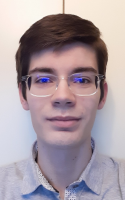
\includegraphics[scale=.5]{imgAA2}

\end{tabular}

\vspace*{-18mm}
\textcolor{maCouleur}{\hfill \begin{tabular}{r}5 Bis rue Mademoiselle Carpentier,\\ 62410 Hulluch - France \\ \ding{38} 06 07 41 87 59,\\ antoine-alexis\_bourdon@ens.univ-artois.fr
  \end{tabular}
}

\vspace*{0.5cm}

\newcommand{\rub}[1]{\vspace*{8mm}{\bf #1}}

%\vspace*{0.1cm}
\addcontentsline{toc}{subsection}{\protect\numberline{1.3} Formation}
\noindent\begin{tabular}{rp{15cm}}
\textcolor{maCouleur}{\rule{2cm}{0.2cm}}& \textcolor{maCouleur}{Formation}\\

depuis 2020 & {\titreligneCV{Master en Informatique}}\\
& Université d'Artois, Faculté des Sciences Jean-Perrin de Lens, Pas-de-Calais, France\\

2017 \--- 2020 & {\titreligneCV{Licence de Mathématiques et Informatique, spécialité Informatique}}\\
& Université d'Artois, Faculté des Sciences Jean-Perrin de Lens, Pas-de-Calais, France\\
& \ding{227} Initiation aux réseaux \\
& \ding{227} Langage: Python, C, HTML5, CSS3, JavaScript, Java, SQLite3, Assembleur, Haskell \\[1mm]
\vspace*{-0.5cm}\\
\end{tabular}

\noindent\begin{tabular}{rp{15cm}}
\textcolor{maCouleur}{\rule{2cm}{0.2cm}}&\textcolor{maCouleur}{Expériences}\\

 2019 & {\textbf{Creator Days (Hackathon)}, Arras, Pas-de-Calais, France \newline
{\scriptsize Évènement de 36H pendant lequel nous devons répondre à une problématique donnée par une entreprise.}\newline
\ding{227} Apprendre à travailler avec des gens que l'on ne connaît pas\newline
\ding{227} Avoir une approche du travail en équipe\newline
\ding{227} Identifier les principaux besoins
}\\[2mm]

2014 \--- 2017 & {\textbf{Assistance informatique}, Henin-Beaumont, Pas-de-Calais, France \newline
\ding{227} Mise à jour des logiciels\newline
\ding{227} Déblocage des logiciels\newline
\ding{227} Maintenance de base des logiciels
}\\[2mm]

2014 \--- 2016 & \ding{227} Technicien et webmasters de serveur Minecraft\\[2mm]

2014 & {Installation réseau, Henin-Beaumont, Pas-de-Calais, France \newline
\ding{227} Mise en place de câblage réseau catégorie 6a
}\\

2013 & \ding{227} Stage d’observation chez \textbf{FIDUCIAL INFORMATIQUE}\\
\vspace*{-0.5cm}\\
\end{tabular}

\noindent\begin{tabular}{rp{15cm}}
  \textcolor{maCouleur}{\rule{2cm}{0.2cm}}&\textcolor{maCouleur}{Compétences}\\
  Français & {C2 (langue natale)}\\
  Anglais & {B2}\\
  Informatique & {Microsoft Office; Python, C, HTLM5, PHP7, CSS3, XML, JavaScript, JQuery,
  Assembleur, SQL(Sqlite3, MySQL), Java, Shell, NodeJs, Angular, NoSQL(mongoDB), Latex}\\
  OS & {Linux, Windows}\\
  %d'exploitation &{} \\[2mm]
  Permis & {Catégorie B}\\
  \vspace*{-0.5cm}\\
  \end{tabular}

\noindent\begin{tabular}{rp{15cm}}
  \textcolor{maCouleur}{\rule{2cm}{0.2cm}}&\textcolor{maCouleur}{Centre d'intérêt}\\
  Musique & {Pratique musicale depuis 2014(chant, participation au “prodige”juin 2017)}\\
  Jeux-Vidéos & {RPG; Action; Aventure; Science-Fiction}\\
  Sport & {Natation}\\[6mm]

  %\begin{localsize}
  & \hspace*{1.0cm}\href{http://github.com/antoinealexisb}
         {
\includegraphics[width=0.04\textwidth]{git}} \hspace*{2.8cm} \href{http://www.linkedin.com/in/antoinealexisb}{
\includegraphics[width=0.04\textwidth]{linke}}\\
  & \href{http://github.com/antoinealexisb}{\tiny github.com/antoinealexisb} \href{http://www.linkedin.com/in/antoinealexisb}{\tiny \ \ \ linkedin.com/in/antoinealexisb}
  %\end{localsize}
  \end{tabular}

  %\begin{figure}
   % \href{http://commons.wikimedia.org/wiki/File:Pachydyptes_ponderosus.jpg}
    %     {
\includegraphics[width=0.1\textwidth]{git}}
    %\caption{A reconstruction of New Zealand Giant Penguins (\emph{pachydyptes ponderosus}) by
    %  F.~W.~Kuhnert (1865--1926). Click on the image to visit the page on Wikimedia Commons where it
    %  was downloaded from.}
  %\end{figure}

\end{document}%  LocalWords:  t'il
